\documentclass[a4paper,landscape,9pt]{article}

\usepackage[margin=1cm]{geometry}
\usepackage{fontspec}
\setmainfont{TeX Gyre Pagella}
\usepackage{unicode-math}
\setmathfont{TeX Gyre Pagella Math}

\usepackage{tikz}
\usetikzlibrary{arrows.meta,calc,positioning,shapes.geometric}
\usepackage{microtype}

\pagestyle{empty}
\setlength{\parindent}{0pt}
\setlength{\parskip}{0.2em}

\tikzset{
  node-d/.style={draw,fill=black,regular polygon,regular polygon sides=6,minimum size=6mm,inner sep=0pt,text=white,font=\tiny\bfseries},
  node-a/.style={draw,fill=black!70,regular polygon,regular polygon sides=3,minimum size=6mm,inner sep=0pt,text=white,font=\tiny\bfseries},
  node-t/.style={draw,circle,minimum size=6mm,inner sep=0pt,line width=0.4pt,font=\tiny},
  node-o/.style={draw,fill=black!15,rectangle,minimum size=6mm,inner sep=0pt,font=\tiny},
  node-i/.style={draw,diamond,minimum size=7mm,inner sep=0pt,line width=0.4pt,font=\tiny},
  impl/.style={-{Latex[length=1.2mm]},line width=0.3pt,black!80},
  exemp/.style={-{Latex[length=1.2mm]},line width=0.3pt,dashed,black!80},
  equiv/.style={{Latex[length=1.2mm]}-{Latex[length=1.2mm]},line width=0.5pt,double,double distance=0.7pt},
  band/.style={font=\scriptsize\scshape,text=black!60},
  bandline/.style={draw,black!18,line width=0.3pt},
}

\begin{document}

\begin{center}
{\large\scshape Proposisjonsgraf, seksjon 5}\hspace{0.8em}{\itshape Verda rommar agentar som responderer på landskapet}
\end{center}

\vspace{-0.5em}

\begin{center}
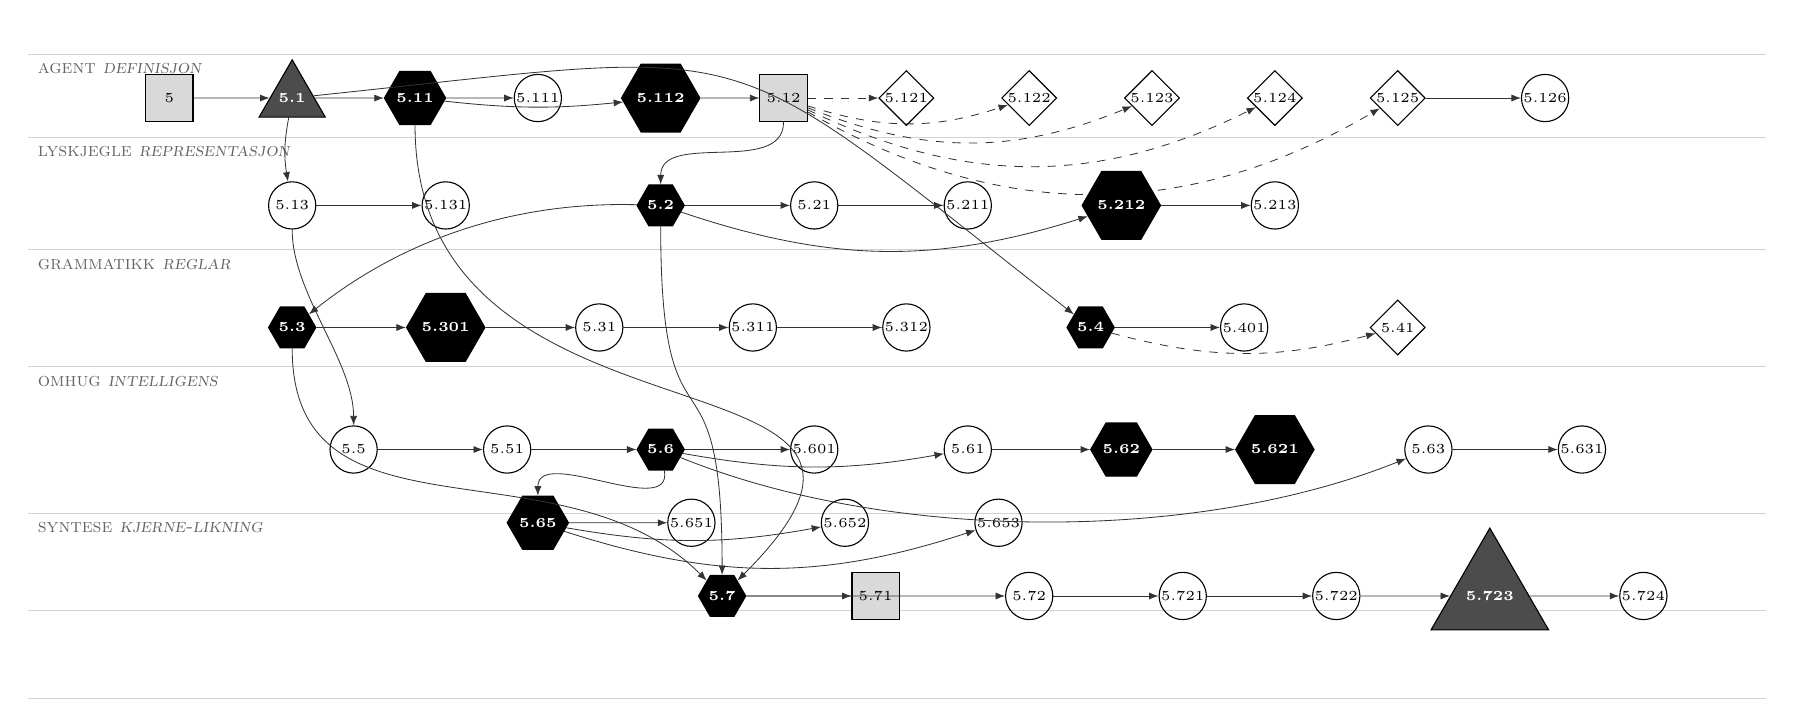
\begin{tikzpicture}[x=0.78cm,y=0.62cm]

  \draw[bandline] (-0.3, 0.6)  -- (28, 0.6);
  \draw[bandline] (-0.3, -1.1) -- (28, -1.1);
  \draw[bandline] (-0.3, -3.4) -- (28, -3.4);
  \draw[bandline] (-0.3, -5.8) -- (28, -5.8);
  \draw[bandline] (-0.3, -8.8) -- (28, -8.8);
  \draw[bandline] (-0.3, -10.8)-- (28, -10.8);
  \draw[bandline] (-0.3, -12.6)-- (28, -12.6);

  \node[band,anchor=west] at (-0.3, 0.3)  {agent  \itshape definisjon};
  \node[band,anchor=west] at (-0.3, -1.4) {lyskjegle  \itshape representasjon};
  \node[band,anchor=west] at (-0.3, -3.7) {grammatikk  \itshape reglar};
  \node[band,anchor=west] at (-0.3, -6.1) {omhug  \itshape intelligens};
  \node[band,anchor=west] at (-0.3, -9.1) {syntese  \itshape kjerne-likning};

  % BAND 1: agent (definisjon og stratifisering)
  \node[node-o] (p5)     at (2, -0.3)    {5};
  \node[node-a] (p51)    at (4, -0.3)    {5.1};
  \node[node-d] (p511)   at (6, -0.3)    {5.11};
  \node[node-t] (p5111)  at (8, -0.3)    {5.111};
  \node[node-d] (p5112)  at (10, -0.3)   {5.112};
  \node[node-o] (p512)   at (12, -0.3)   {5.12};
  \node[node-i] (p5121)  at (14, -0.3)   {5.121};
  \node[node-i] (p5122)  at (16, -0.3)   {5.122};
  \node[node-i] (p5123)  at (18, -0.3)   {5.123};
  \node[node-i] (p5124)  at (20, -0.3)   {5.124};
  \node[node-i] (p5125)  at (22, -0.3)   {5.125};
  \node[node-t] (p5126)  at (24.4, -0.3) {5.126};
  \draw[impl] (p5)   -- (p51);
  \draw[impl] (p51)  -- (p511);
  \draw[impl] (p511) -- (p5111);
  \draw[impl] (p511) to[bend right=6] (p5112);
  \draw[impl] (p5112) -- (p512);
  \draw[exemp] (p512) -- (p5121);
  \draw[exemp] (p512) to[bend right=18] (p5122);
  \draw[exemp] (p512) to[bend right=22] (p5123);
  \draw[exemp] (p512) to[bend right=26] (p5124);
  \draw[exemp] (p512) to[bend right=30] (p5125);
  \draw[impl] (p5125) -- (p5126);

  % BAND 2: lyskjegle (representasjon og grense)
  \node[node-t] (p513)   at (4, -2.5)    {5.13};
  \node[node-t] (p5131)  at (6.5, -2.5)  {5.131};
  \node[node-d] (p52)    at (10, -2.5)   {5.2};
  \node[node-t] (p521)   at (12.5, -2.5) {5.21};
  \node[node-t] (p5211)  at (15, -2.5)   {5.211};
  \node[node-d] (p5212)  at (17.5, -2.5) {5.212};
  \node[node-t] (p5213)  at (20, -2.5)   {5.213};
  \draw[impl] (p51)   to[bend right=10] (p513);
  \draw[impl] (p513)  -- (p5131);
  \draw[impl] (p512)  to[out=-90,in=90] (p52);
  \draw[impl] (p52)   -- (p521);
  \draw[impl] (p521)  -- (p5211);
  \draw[impl] (p52)   to[bend right=18] (p5212);
  \draw[impl] (p5212) -- (p5213);

  % BAND 3: grammatikk og substrat
  \node[node-d] (p53)    at (4, -5)      {5.3};
  \node[node-d] (p5301)  at (6.5, -5)    {5.301};
  \node[node-t] (p531)   at (9, -5)      {5.31};
  \node[node-t] (p5311)  at (11.5, -5)   {5.311};
  \node[node-t] (p5312)  at (14, -5)     {5.312};
  \node[node-d] (p54)    at (17, -5)     {5.4};
  \node[node-t] (p5401)  at (19.5, -5)   {5.401};
  \node[node-i] (p541)   at (22, -5)     {5.41};
  \draw[impl] (p52)    to[bend right=20,looseness=0.9] (p53);
  \draw[impl] (p53)    -- (p5301);
  \draw[impl] (p5301)  -- (p531);
  \draw[impl] (p531)   -- (p5311);
  \draw[impl] (p5311)  -- (p5312);
  \draw[impl] (p51)    to[bend left=22,looseness=1.5] (p54);
  \draw[impl] (p54)    -- (p5401);
  \draw[exemp] (p54)   to[bend right=15] (p541);

  % BAND 4: omhug og kompetanse
  \node[node-t] (p55)    at (5, -7.5)    {5.5};
  \node[node-t] (p551)   at (7.5, -7.5)  {5.51};
  \node[node-d] (p56)    at (10, -7.5)   {5.6};
  \node[node-t] (p5601)  at (12.5, -7.5) {5.601};
  \node[node-t] (p561)   at (15, -7.5)   {5.61};
  \node[node-d] (p562)   at (17.5, -7.5) {5.62};
  \node[node-d] (p5621)  at (20, -7.5)   {5.621};
  \node[node-t] (p563)   at (22.5, -7.5) {5.63};
  \node[node-t] (p5631)  at (25, -7.5)   {5.631};
  % Liv-subkaskaden: plassert i eiga underrad nedanfor, offset for å unngå visuell stacking
  \node[node-d] (p565)   at (8, -9)      {5.65};
  \node[node-t] (p5651)  at (10.5, -9)   {5.651};
  \node[node-t] (p5652)  at (13, -9)     {5.652};
  \node[node-t] (p5653)  at (15.5, -9)   {5.653};
  \draw[impl] (p513)  to[out=-90,in=90,looseness=0.8] (p55);
  \draw[impl] (p55)   -- (p551);
  \draw[impl] (p551)  -- (p56);
  \draw[impl] (p56)   -- (p5601);
  \draw[impl] (p56)   to[bend right=10] (p561);
  \draw[impl] (p561)  -- (p562);
  \draw[impl] (p562)  -- (p5621);
  \draw[impl] (p56)   to[bend right=22,looseness=0.8] (p563);
  \draw[impl] (p563)  -- (p5631);
  \draw[impl] (p56)   to[out=-80,in=90] (p565);
  \draw[impl] (p565)  -- (p5651);
  \draw[impl] (p565)  to[bend right=10] (p5652);
  \draw[impl] (p565)  to[bend right=18] (p5653);

  % BAND 5: syntese (kjerne-likning, reduksjonsteorem og lukking)
  \node[node-d] (p57)    at (11, -10.5)  {5.7};
  \node[node-o] (p571)   at (13.5, -10.5)  {5.71};
  \node[node-t] (p572)   at (16, -10.5)  {5.72};
  \node[node-t] (p5721)  at (18.5, -10.5)  {5.721};
  \node[node-t] (p5722)  at (21, -10.5)  {5.722};
  \node[node-a] (p5723)  at (23.5, -10.5){5.723};
  \node[node-t] (p5724)  at (26, -10.5){5.724};
  \draw[impl] (p53)   to[out=-90,in=135,looseness=1.1] (p57);
  \draw[impl] (p52)   to[out=-90,in=90,looseness=1.8] (p57);
  \draw[impl] (p511)  to[out=-90,in=45,looseness=1.6] (p57);
  \draw[impl] (p57)   -- (p571);
  \draw[impl] (p57)   -- (p572);
  \draw[impl] (p572)  -- (p5721);
  \draw[impl] (p5721) -- (p5722);
  \draw[impl] (p5722) -- (p5723);
  \draw[impl] (p5723) -- (p5724);

\end{tikzpicture}
\end{center}

\vspace{-0.2em}

\hrule

\vspace{0.3em}

\begin{minipage}[t]{0.325\textwidth}
{\scshape\small Lesing ovanfrå}

Seksjon 5 opnar med postulatet \emph{5.1} (triangel): kvar klasse har minst eitt system som navigerer landskapet via negativ tilbakekopling. Frå dette bygger \emph{5.11} den substrat-uavhengige definisjonen av \textbf{agent} som tuppelet $(m,\pi,\varepsilon)$: generativ modell, politikk som minimerer fri energi, og toleranseterskel for KL-divergens. \emph{5.112} legg til \textbf{prediksjonshorisont} $\tau(A)$.

Band 1 er stratifisert langs fem illustrasjonar (romber \emph{5.121} til \emph{5.125}): termostat, tre, koloni, pattedyr, designar. Designaren sin særprega posisjon står i \emph{5.126}: han navigerer på vegne av andre.

Band 2 introducerer \textbf{kognitiv lyskjegle} (\emph{5.2}) med formell KL-divergens\-definisjon (\emph{5.212}); lyskjegla fell direkte ut av agentdefinisjonen.
\end{minipage}\hfill
\begin{minipage}[t]{0.325\textwidth}
{\scshape\small Lesing nedover}

Band 3 spaltar seg i to: formgrammatikken (\emph{5.3, 5.301}) til venstre, substratet som null-ordens agent (\emph{5.4}) til høgre. \emph{5.41} illustrerer: bioelektrisk polarisering, materiell friksjon, vektoriell merksemd; same struktur, ulike substrat.

Band 4 er seksjonens rikaste band statistisk. \textbf{Kapasitet} C(A) (\emph{5.601}) og \textbf{omhug} $\omega(A)$ (\emph{5.6}) står no som vektor-storleikar: kapasiteten er mengda av aksar agenten \emph{kan} halde under $\varepsilon$; omhug er fordelinga over kor nær politikken faktisk kjem terskelen per akse. Spesialist og generalist er to profilar av same vektor. K-metrikken (\emph{5.621}) står vidare som kvantitativ kompetansemål. Liv-definisjonen (\emph{5.65}) hengjer ned som eigen underseksjon.

Band 5 er syntesepunktet. \emph{5.7} er kjerne-likninga, og han har \emph{tre foreldre}: agentar, lyskjegle, grammatikk. \emph{5.724} lukkar: $\mathbb{M}$ og $\Pi$ er avleidde frå dei tre laga.
\end{minipage}\hfill
\begin{minipage}[t]{0.325\textwidth}
{\scshape\small Strukturelle innsikter}

\emph{Tripleteforeldreskap.} \emph{5.7} er den einaste noden i traktaten med tre direkte foreldre. Dette er oppfinningssjangerens høgdepunkt.

\emph{FEP-reduksjon.} Agentdefinisjonen i \emph{5.11} er no ein rein Friston-formulering: (m,\,$\pi$,\,$\varepsilon$). Dei eldre formalismane (Rosenblueth-Wiener-Ashby, RL) er spesialtilfelle. Fire tradisjonar konvergerer.

\emph{Omhug som fordeling.} F3 i endringsplanen er løyst: omhug er ikkje skalar, men vektor. Sviktsignatur kan lesast per akse.

\emph{Dobbel lukking.} \emph{5.723} (meta: feltet lukkar) og \emph{5.724} (ontologi/epistemologi: $\mathbb{M}$ og $\Pi$ er avleidde) står saman i band 5.

\emph{Fem illustrasjonar.} Flest romber i nokon seksjon. Stratifiseringa frå termostat til designar er visuelt kompakt i éi rekke.

\emph{Sjanger stadfesta.} Oppfinningseksjonane (1, 2, 5, 6) har alle konfluens.
\end{minipage}

\end{document}
